\section{División de Bienes}

Una de las parejas más ricas del mundo está pasando por un proceso de divorcio. Entre sus bienes cuentan con propiedades, autos, motos, estampillas raras y otros coleccionables. Como no se ponen de acuerdo en la manera de dividirlos, el juez ha dictaminado que un tasador ponga valor a cada bien y luego se haga una partición por valores iguales. El juez nos pide que elaboremos un algoritmo que en forma eficiente haga este trabajo.\newline
%============================================

\subsection{Solución}
El problema que precede se puede pensar como una representación de un conjunto

$C=\{w_{1}, w_{2}, ..., w_{n}\}$ donde cada $w_{i}$ está asociado al precio de cada bien. Luego, se desea determinar si existe un subconjunto de C tal que:

\begin{equation}
    W=\sum w_{i}
\end{equation}

Donde $w_{i}$ representa el precio de cada bien.

Utilizando conceptos de programación dinámica es posible llegar a una solución. No obstante, dicha solución estaría caracterizada por ser $O(W\cdot n)$, donde n es la cantidad de bienes y W es el valor de la ecuación (1) al que se desea llegar. Esto puede llegar a ser de orden casi exponencial si considera un W muy grande, y se tiene en cuenta la cantidad de bits empleados para representarlo y su crecimiento.

Sin embargo, como se describirá en el siguiente apartado, el problema es NP-Completo, de manera que no es posible hallar una solución que no sea exponencial. Al menos así ha sido descripto hasta ahora.

\subsection{Demostración NP-C}
%=============================================
Para poder demostrar que el problema es NP-Completo, se decidió proceder realizando la demostración a partir de dos hipótesis:
\begin{itemize}
    \item El problema es NP
    \item El problema es NP-Hard
\end{itemize}

Si ambas se cumplen, podemos afirmar que el problema es NP-Completo.

En primer lugar, se debe demostrar que es NP. Utilizando la notación previa, se puede decir que el subconjunto C puede tener tantos elementos como el conjunto original. Para poder hallar a W es preciso realizar las sumas asociadas a las iteraciones de los diferentes $w_{i}$. Esto se puede resolver en tiempo polinomial, luego el problema es NP.

Ahora se debe probar que el problema es NP-Hard. 

Para eso se va a demostrar:

\begin{equation}
    3DM \leq_{p} SUBSET-SUM
\end{equation}

La demostración se sustenta en que es conocido que el problema 3 dimensional matching es NP-C.

Para proceder a demostrar que el problema SUBSET SUM se puede reducir a 3DM se planteará que el conjunto C $\subseteq X,Y,Z$, siendo estos conjuntos ordenados disjuntos de tamaño n cada uno. Se desea determinar si existe el conjunto C.

Luego, se procede a representar a una tripla $t={x_{i}, y_{i}, z_{i}}$ como una serie de bits de tamaño 3n. A los efectos de resolver el problema se plantea que el conjunto C se puede representar como se demuestra a continuación:

\begin{figure}[H]
\centering
\includegraphics[width=0.7\textwidth]{Informe/Imagenes/Parte2/imagen1.png}
\caption{\label{fig:class01}Representación de tripla}
\end{figure}

No obstante, esta representación trae aparejado un posible problema de overflow. Esto se puede observar en la siguiente representación:

\begin{figure}[H]
\centering
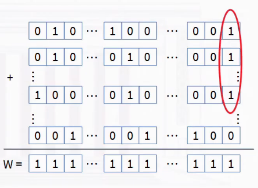
\includegraphics[width=0.5\textwidth]{Informe/Imagenes/Parte2/imagen2.png}
\caption{\label{fig:class01}Problema de overflow}
\end{figure}

Para evitar esta situación se debe elegir una representación en una base al menos un valor mayor de la cantidad de triplas, ya que esto imposibilita que se presente el overflow.

Al llegar a una representación del problema que se puede caracterizar por 3DM, podemos afirmar que el mismo representa a un problema similar a 3DM. 

Por lo tanto, como 3DM es NP-C, se probó la ecuación (2) y también que el problema es NP, se puede afirmar que se trata de un problema NP-C.